%%%%%%%%%%%%%%%%%%%%%%%%%%%%%%%%%%%%%%%%%
% University/School Laboratory Report
% LaTeX Template
% Version 3.1 (25/3/14)
%
% This template has been downloaded from:
% http://www.LaTeXTemplates.com
%
% Original author:
% Linux and Unix Users Group at Virginia Tech Wiki 
% (https://vtluug.org/wiki/Example_LaTeX_chem_lab_report)
%
% License:
% CC BY-NC-SA 3.0 (http://creativecommons.org/licenses/by-nc-sa/3.0/)
%
%%%%%%%%%%%%%%%%%%%%%%%%%%%%%%%%%%%%%%%%%

%----------------------------------------------------------------------------------------
%	PACKAGES AND DOCUMENT CONFIGURATIONS
%----------------------------------------------------------------------------------------

\documentclass{article}

\usepackage[version=3]{mhchem} % Package for chemical equation typesetting
\usepackage{siunitx} % Provides the \SI{}{} and \si{} command for typesetting SI units
\usepackage{graphicx} % Required for the inclusion of images
\usepackage{natbib} % Required to change bibliography style to APA
\usepackage{amsmath} % Required for some math elements 
\usepackage{bm}
\usepackage{amssymb}
\setlength\parindent{0pt} % Removes all indentation from paragraphs

\renewcommand{\labelenumi}{\alph{enumi}.} % Make numbering in the enumerate environment by letter rather than number (e.g. section 6)

\usepackage{times} % Uncomment to use the Times New Roman font
\usepackage{verbatim}
\usepackage{tabulary}
\usepackage{algorithmic}
\usepackage{algorithm}
%----------------------------------------------------------------------------------------
%	DOCUMENT INFORMATION
%----------------------------------------------------------------------------------------

\title{NYU-MMVC-LAB Weekly Report} % Title

\author{Jing \textsc{Zhu}} % Author name

\date{\today} % Date for the report
%\date{September 13, 2015}

\begin{document}

\maketitle % Insert the title, author and date

%\begin{center}
%\begin{tabular}{l r}
%Date Performed: & January 1, 2012 \\ % Date the experiment was performed
%Partners: & James Smith \\ % Partner names
%& Mary Smith \\
%Instructor: & Professor Smith % Instructor/supervisor
%\end{tabular}
%\end{center}

% If you wish to include an abstract, uncomment the lines below
% \begin{abstract}
% Abstract text
% \end{abstract}

%----------------------------------------------------------------------------------------
%	SECTION 1
%----------------------------------------------------------------------------------------

\section{Motivation}
Since the efficient and effective backpropagation algorithm was proposed, neural network becomes much more popular for machine learning problems, especially for classification problems.  \\   

We aim to learn an effective cross-domain non-linear distance metric for depth image-based 3D model retrieval. By minimizing the within-class distances and maximizing the between-class distances for the outputs of the metric networks, we develop a novel pairwise metric learning network to learn a non-linear transformation to retrieve 3D models based on depth image queries.\\

In this week, we analyze the derivation of back propagation and conduct experiments on the NYU Depth V2 dataset and the SHREC 2014 benchmark.

\begin{figure}[t]
	
	\centering
	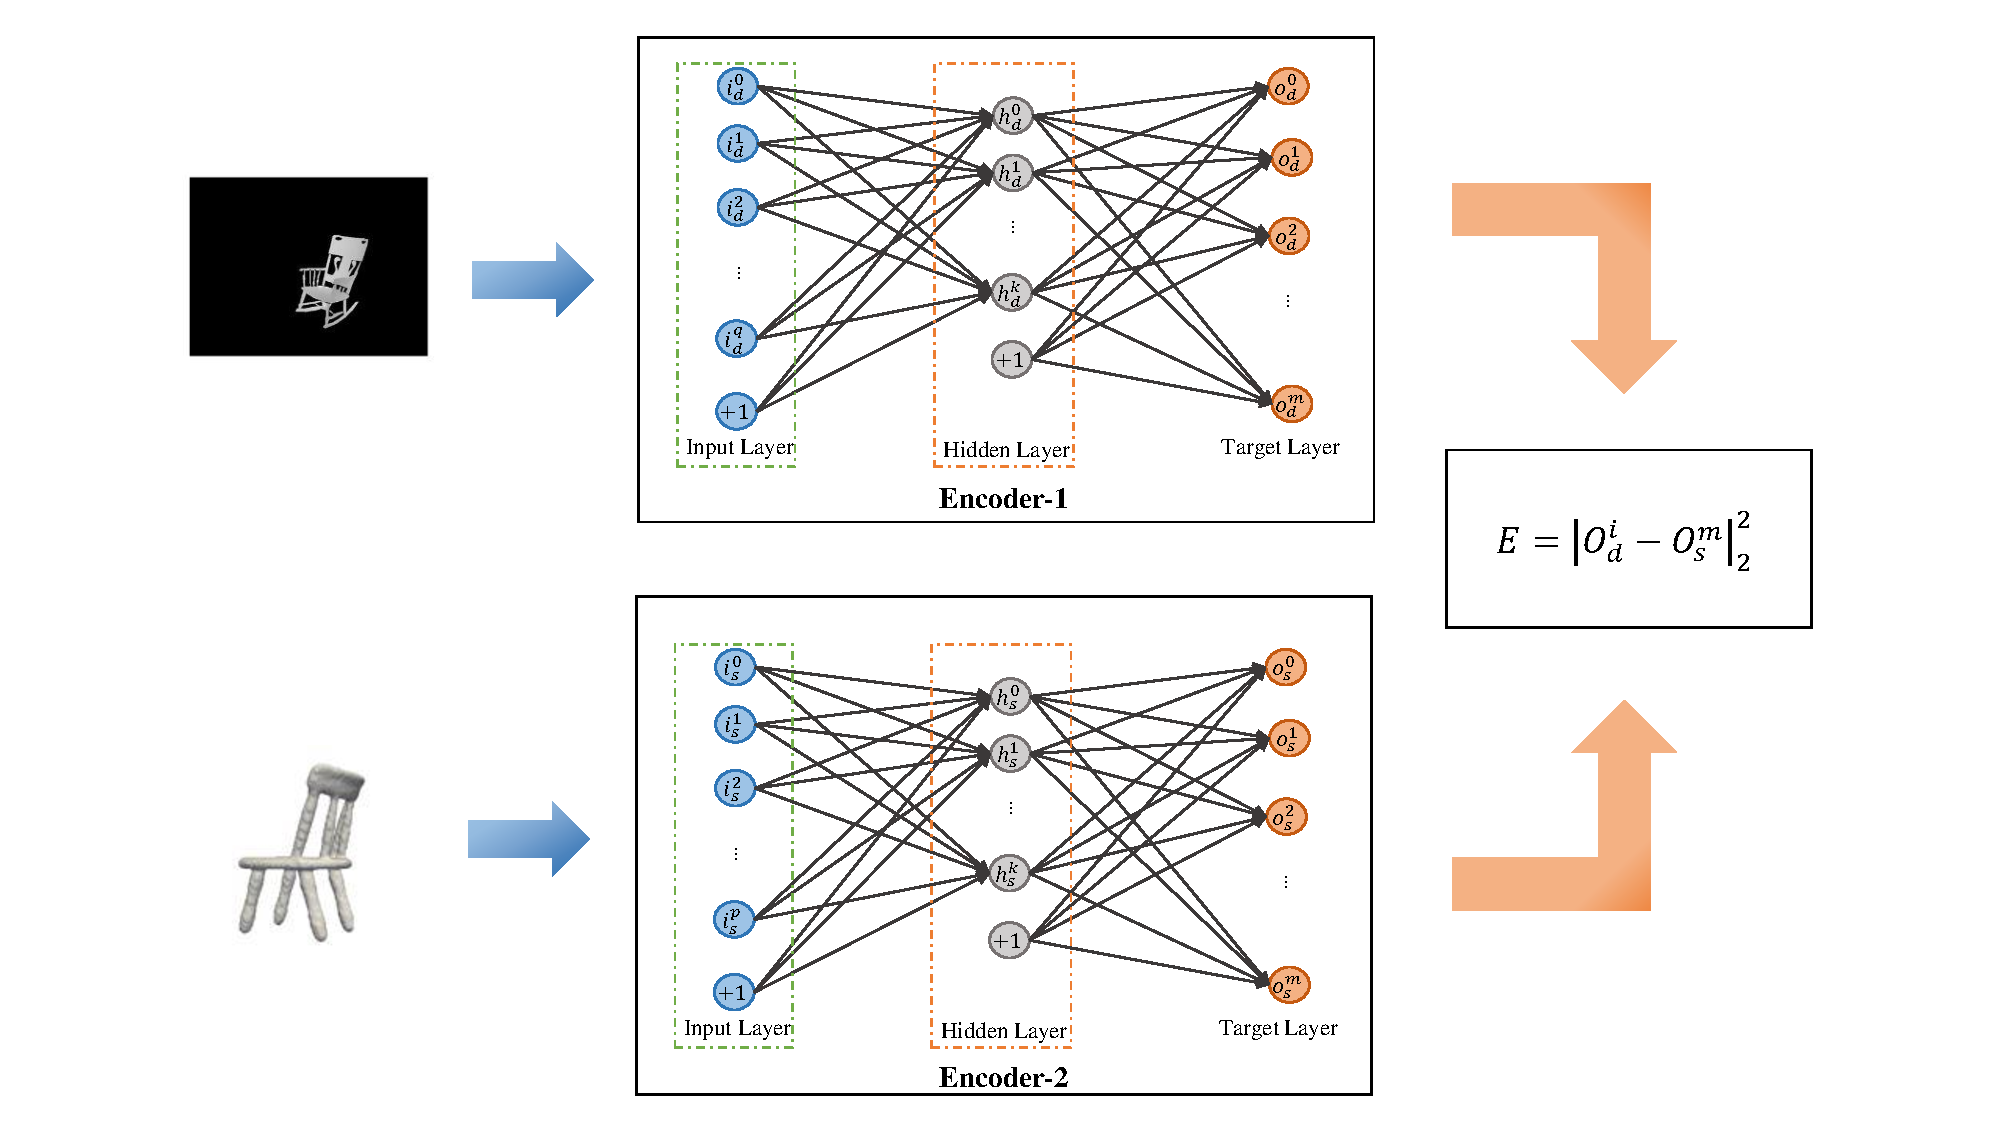
\includegraphics[height=7cm, width=12cm]{figure.pdf}
	\caption{The framework of our proposed pairwise metric learning network}
	%\vspace{-0.3cm}
	\label{figure1}
\end{figure}

%----------------------------------------------------------------------------------------
%	SECTION 2
%----------------------------------------------------------------------------------------


\section{Methods}
In general, neural networks are trained only based on within-class distance. In our past research work, we have tried to train a pairwise neural network for the depth image-based 3D shape retrieval, however, we did not get a really good performance by using two 3-layer neural network. Therefore, it would be more reliable and desirable that between-class distance is taken into consideration. \\

As shown in Figure \ref{figure1}, two 3-layer neural networks are exploited for our task. One takes extraced ScSPM features from depth image as input and the other takes extracted 3D SIFT features from 3D models as input. We define the error function based on the outputs from both 3D neural network and depth neural network and apply popular backpropagation by minimizing the value of error function. Detailed derivation process will be given in Implementation section.\\


%----------------------------------------------------------------------------------------
%	SECTION 3
%----------------------------------------------------------------------------------------

\vspace{0.3cm}
\section{Implementation}
We consider a 3-layer neural network, which has an input layer, a hidden layer and a target layer.   We adopt sigmoid function $f(z)$ as activation function for each neuron in our neural network: 
\begin{equation}
f(z)=\frac{1}{1+exp(-z)}.
\end{equation}\\
The activations of layer $k$ from the pairwise neural network are denoted as  $a_d^k$ and $a_s^k$, respectively:
\begin{equation}
	\begin{aligned}
		a_{d}^{k+1} &= f(W_d^ka_d^k + b_d^k)=f(r_{d}^{k+1})\\
		a_{s}^{k+1} &= f(W_s^ka_s^k + b_s^k)=f(r_{s}^{k+1})\\
	\end{aligned}
	\label{trans1}
\end{equation}
where $r_{d}^{k+1}=W_d^ka_d^k + b_d^k$ and $r_{s}^{k+1}=W_s^ka_s^k + b_s^k$. Let $\bm{O}^{i}_{d}=\{ \bm{o}^{0}_{d}, \bm{o}^{1}_{d}, \bm{o}^{2}_{d},\cdots, \bm{o}^{M_{d}}_{d} \} \in \mathbf{R}^{N_{d} \times M_{d}}$ and $\bm{O}^{i}_{s}=\{ \bm{o}^{0}_{s}, \bm{o}^{1}_{s}, \bm{o}^{2}_{s},\cdots, \bm{o}^{M_{s}}_{s}\} \in \mathbf{R}^{N_{s} \times M_{s}}$ be output values at the $K^{th}$ layer (in our case, $K=3$) based on the depth ($\bm{I}^{i}_{d}$) and 3D model domain inputs ($\bm{I}^{i}_{s}$) respectively. Then, 
\begin{equation}
	\begin{aligned}
		O_{d}^{i} = a_{d}^{K}	&& O_{s}^{i} &= a_{s}^{K}.\\
	\end{aligned}
	\label{trans2}
\end{equation}



A unified objective function for learning the pairwise neural networks can be formulated as:

\begin{equation}
\label{eq5}
\begin{aligned}
E(W_{d}, b_{d},W_{s}, b_{s})=\operatorname*{arg\,min}_{\bm{W_d},\bm{b_d},\bm{W_s},\bm{b_s}}&\frac{1}{N_{1}}\sum_{i=1}^{M_d}\sum_{j=1,C(j)=C(i)}^{M_s}\frac{1}{2}\|\bm{o_d}^i- \bm{o_s}^j\|_2^2 - \frac{1}{N_{2}}\sum_{i=1}^{M_d}\sum_{j=1,C(j)\neq C(i)}^{M_s}\frac{1}{2}\|\bm{o_d}^i - \bm{o_s}^j\|_2^2\\+\frac{1}{2}\lambda\sum_{l=1}^2(\|\bm{W_d}^l\|_F^2+\|\bm{W_s}^l\|_F^2),\\
\end{aligned}
\end{equation} 
\\
We adopt the back-propagation algorithm to optimize each term in the objective function  Eq.\ref{eq5}. The derivative of the objective function $E$ with respect to $W_d^k$, $b_d^k$, $W_s^k$ and $b_s^k$ are denoted as $\frac{\partial E}{\partial W_d^k}$, $\frac{\partial E}{\partial b_d^k}$, $\frac{\partial E}{\partial W_s^k}$, $\frac{\partial E}{\partial b_s^k}$. Taking $\frac{\partial E}{\partial W_d^k}$ and $\frac{\partial E}{\partial W_s^k}$ as an example, $\frac{\partial E}{\partial b_d^k}$ and $\frac{\partial E}{\partial b_s^k}$ could be derived similarly.Let $E_1 = \frac{1}{2}\|\bm{o_d}^i- \bm{o_s}^j\|_2^2$. Then, \\

\begin{equation}
	\begin{aligned}
		\frac{\partial E}{\partial W_d^k} =&\frac{1}{N_{1}}\sum_{i=1}^{M_d}\sum_{j=1,C(j)=C(i)}^{M_s}\frac{\partial E_1 }{\partial W_d^k} - \frac{1}{N_{2}}\sum_{i=1}^{M_d}\sum_{j=1,C(j)=C(i)}^{M_s}\frac{\partial E_1}{\partial W_d^k} + \lambda W_d^k
	\end{aligned}
	\label{allupdate1}
\end{equation}
\\
\begin{equation}
\begin{aligned}
	\frac{\partial E}{\partial W_s^k} =&\frac{1}{N_{1}}\sum_{i=1}^{M_d}\sum_{j=1,C(j)=C(i)}^{M_s}\frac{\partial E_1 }{\partial W_s^k} - \frac{1}{N_{2}}\sum_{i=1}^{M_d}\sum_{j=1,C(j)=C(i)}^{M_s}\frac{\partial E_1}{\partial W_s^k} + \lambda W_s^k .
\end{aligned}
\label{allupdate3}
\end{equation}
\\
$\frac{\partial E_1 }{\partial W_d^k}$ and $\frac{\partial E_1}{\partial W_s^k}$ can be rewritten as:

\begin{equation}
	\begin{aligned}
	\frac{\partial E_1 }{\partial W_d^k} =\frac{\partial E_1 }{\partial r_{d}^{k+1}}\frac{\partial r_{d}^{k+1}}{\partial W_d^k} = \frac{\partial E_1 }{\partial r_{d}^{k+1}}(a_d^k)^{T},  
	\end{aligned}
	\label{eq7}
\end{equation}
\begin{equation}
	\begin{aligned}
	\frac{\partial E_1 }{\partial W_s^k} =&\frac{\partial E_1 }{\partial r_{s}^{k+1}}\frac{\partial r_{s}^{k+1}}{\partial W_s^k}=\frac{\partial E_1 }{\partial r_{s}^{k+1}}(a_s^k)^{T}.   
	\end{aligned}
\label{eq8}
\end{equation}
\\

For $k=K-1$, $\frac{\partial E_1 }{\partial r_{d}^{k+1}}$ and $\frac{\partial E_1 }{\partial r_{s}^{k+1}}$ can be represented as:
\begin{equation}
	\begin{aligned}
	\frac{\partial E_1 }{\partial r_{d}^{k+1}} =&(a_d^K-a_d^K)\bullet f^{'}(r_d^K)\\
	\frac{\partial E_1 }{\partial r_{s}^{k+1}} =&(a_d^K-a_s^K)\bullet f^{'}(r_d^K),   
	\end{aligned}
\end{equation}
\\
where $f^{'}(r_d^K)$ is the derivative of the activation function in the output layer and $\bullet$ denotes the element-wise multiplication. For layer $k=1, 2, \cdots, K-3, K-2$, with the backpropagation algorithm, $\frac{\partial E_1 }{\partial r_{d}^{k+1}}$ and $\frac{\partial E_1 }{\partial r_{s}^{k+1}}$ can be obtained as:
\begin{equation}
	\begin{aligned}
	\frac{\partial E_1 }{\partial r_{d}^{k+1}} =\frac{\partial E_1 }{\partial r_{d}^{k+2}}\frac{\partial r_{d}^{k+2}}{\partial r_{d}^{k+1}}=(W_d^{k+1})^T\frac{\partial E_1 }{\partial r_{d}^{k+2}}\bullet f^{'}(r_d^{k+1}) \\
	 \frac{\partial E_1 }{\partial r_{s}^{k+1}} =\frac{\partial E_1 }{\partial r_{s}^{k+2}}\frac{\partial r_{s}^{k+2}}{\partial r_{s}^{k+1}}=(W_s^{k+1})^T\frac{\partial E_1 }{\partial r_{s}^{k+2}}\bullet f^{'}(r_s^{k+1})  
	\end{aligned}
\end{equation}
\\
Similarly, $\frac{\partial E}{\partial b_d^k}$ and $\frac{\partial E}{\partial b_s^k}$ can be calculated as:
\begin{equation}
	\begin{aligned}
	\frac{\partial E}{\partial b_d^k}=\frac{\partial E_1 }{\partial r_{d}^{k+1}}\frac{\partial r_{d}^{k+1}}{\partial b_d^k}=\frac{\partial E_1 }{\partial r_{d}^{k+1}}\\
	\frac{\partial E}{\partial b_s^k}=\frac{\partial E_1 }{\partial r_{s}^{k+1}}\frac{\partial r_{s}^{k+1}}{\partial b_s^k}=\frac{\partial E_1 }{\partial r_{s}^{k+1}}\\
	\end{aligned}
\label{eq11}
\end{equation}
\\
By substituting Eq.(\ref{eq7}) and  (\ref{eq8}) into Eq.(\ref{allupdate1}) and (\ref{allupdate3}), we can obtain the derivative of the objective function $E$ with respective to $W_d^k$ and $W_s^k$. Similarly, with Eq.(\ref{eq11}), we can get the derivative of the objective function $E$ with respective to $b_k^s$ and $b_k^t$. Then $W_d^k$, $W_s^k$, $b_k^s$ and $b_k^t$ can be updated with the gradient descent algorithm (as shown in Algorithm \ref{algorithm: 001}).\\

\begin{algorithm}
%\vspace{-2mm}
\caption {Training algorithm of proposed pairwise neural network}
\label{algorithm: 001}
\textbf{Input:} depth image training set $S$ and 3D model  dataset $D$; layer size $K$ of the neural network; regularization term $\lambda$ ; learning rate $\beta$.

\textbf{Output:} $W_d$, $W_s$, $b_d$ and $b_s$\\

Do
\begin{enumerate}
	\item Compute the outputs of two neural networks with forward propagation for all the training pair-wise example $I^i_d$ and $I_s^i$;
 \item For $k=K-1,K-2,...1$
	Compute $\frac{\partial E}{\partial W_d^k}$, $\frac{\partial E}{\partial b_d^k}$, $\frac{\partial E}{\partial W_s^k}$ and $\frac{\partial E}{\partial b_s^k}$ with Eq.(\ref{allupdate1}) and Eq. (\ref{allupdate3});
\item Update $W_d^k$, $b_d^k$, $W_s^k$ and $b_s^k$ for $k=1,2,...,K-1$:\\
\\
	$W_d^k = W_d^k - \beta \frac{\partial E}{\partial W_d^k},  \quad b_d^k = b_d^k - \beta \frac{\partial E}{\partial b_d^k}$	\\
\\
	$W_s^k = W_s^k - \beta \frac{\partial E}{\partial W_s^k},  \quad b_s^k = b_s^k - \beta \frac{\partial E}{\partial b_s^k}$
\\

\end{enumerate}
Until convergence
\end{algorithm}

%----------------------------------------------------------------------------------------
%	SECTION 4
%----------------------------------------------------------------------------------------

\section{Experimental Results}
The NYU Depth V2 dataset contains frames of video sequences in a variety of indoor scenes, from where objects in depth images are extracted as queries in our experiments. The database is constructed by selecting 3D models in correponding categories from the large-scale extended SHREC 2014 benchmark. The number of samples in 10 categories ({\it bathtub, bed, chair, desk, dresser, monitor, stand, sofa, table, toilet}) of both datasets are given in Table \ref{table1}.
\\
We evaluate the proposed approach using 6 common evaluation metrics, Nearest neighbor (NN), First Tier (FT), Second Tire (ST), E-Measure (E), Discounted Cumulated Gain (DCG) and Average Precision (AP). We conduct experiments using all 10 categories, and compare with the state-of-art transfer learning approaches CM, SCM and PNN. We also compare with the non-transfer (NT) approach, which directly utilizes the original depth image and 3D model representations for retrieval. Results are reported in Table \ref{table2}.

\begin{table}
	
	\footnotesize
	\centering
	\caption{Number of samples of each category in 3D model datasets and depth image dataset}
	\label{table1}
	\begin{tabular}{ccccccccccc}
		\hline
		\hline
		\noalign{\smallskip}
		 &bathtub &bed & chair & desk & dresser & monitor &stand &sofa &table &toilet\\ \hline\noalign{\smallskip}	
		3D model &109 &467 &712 &204 &203 &433 &218 &602 &402 &324\\
		Depth image &57  &318 &654 &197 &111 &118 &148 &307 &539 &68 \\		
		\hline\noalign{\smallskip}	
		\hline
	\end{tabular}
\end{table}

\begin{table}
	
	\footnotesize
	\centering
	\caption{Performance metrics comparison of depth image-based 3D model retrieval on the NYU Depth V2 dataset and the SHREC 2014 benchmark.}
	\label{table2}
	\begin{tabular}{ccccccc}
		\hline
		\hline
		\noalign{\smallskip}
		&NN & FT & ST & DCG & E & AP\\ \hline\noalign{\smallskip}		
		10 categories\\ 
		NT  &0.10 &0.11 &0.23 & 0.67 & 0.01 & 0.13 \\ 
		CM  &0.11 &0.13 &0.25 & 0.67 & 0.02 & 0.13 \\ 
		SCM &0.12 &0.13 &0.25 & 0.67 & 0.02 & 0.13 \\ 
		PNN &0.13 &0.14 &0.27 & 0.68 & 0.02 & 0.14 \\		
		%IPNN &0.03 &0.12 &0.31 &0.56 &0.03 &0.22\\
		Metric Learning &$\bm{0.89}$ &$\bm{0.76}$ &$\bm{0.79}$ &$\bm{0.92}$ &$\bm{0.10}$ &$\bm{0.78}$\\\hline
		\hline
	\end{tabular}
	%\vspace{-0.4cm}
\end{table}

%----------------------------------------------------------------------------------------
%	SECTION 5
%----------------------------------------------------------------------------------------
\section{Conclusion}
As we can see from performance metrics, our new approach achieves better performance on the NYU Depth Dataset V2 and the extended SHREC 2014 3D shape retrieval benchmark.\\
 

%----------------------------------------------------------------------------------------
%	BIBLIOGRAPHY
%----------------------------------------------------------------------------------------
%----------------------------------------------------------------------------------------

\end{document}
